\subsection{DroNet: Learning to Fly by Driving}

In their paper, Loquercio \etal~\cite{dronet}~propose a ResNet with only 8
layers, with an average accuracy only 1\% below ResNet-50 for the same
regression task. The objective function is in fact a combination of two
regressions allowing a drone to navigate in urban environments. Their network,
as seen on Figure~\ref{fig:dronetoriginal}, contains two fully connected
layers: one for the steering commands of the drone, one for the collision
detection probability.

\begin{figure}[h]
	\center
	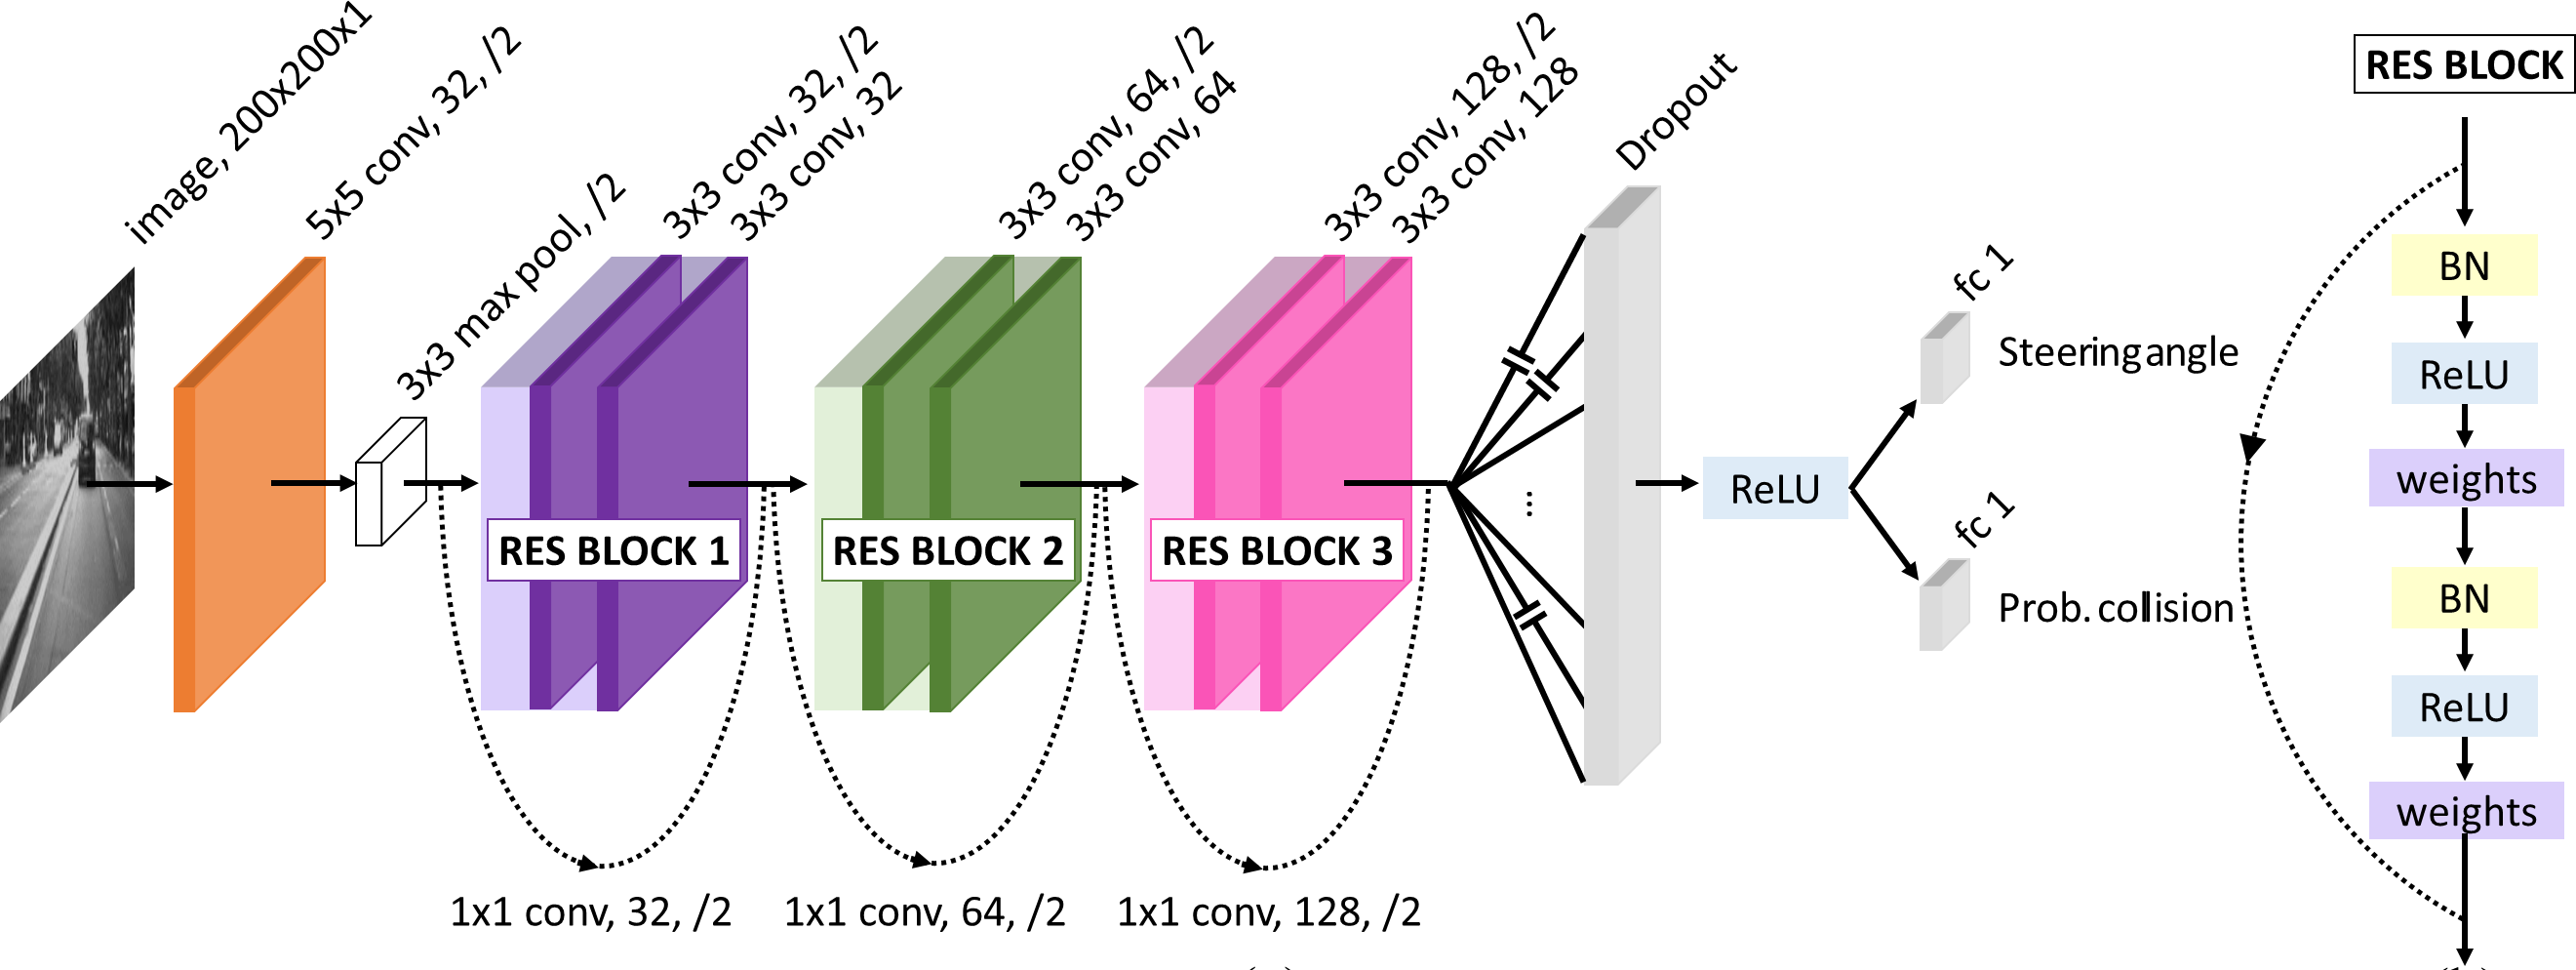
\includegraphics[width=\textwidth]{figure/dronet.png}
	\label{fig:dronetoriginal}
	\caption{The original DroNet model~\cite{dronet}.}
\end{figure}

What makes this model an attractive choice is its impressive performance when
compared to ResNet-50, with only $81\times$ fewer parameters, thus making it
well suited for embedded applications such as drone racing.\\

The network was trained on an outdoor dataset of $70,000$ car driving images
from Udacity's project, as well as a custom bicycle dataset of $32,000$
pictures they have collected for the collision detection. As for the input
specifications, the format used is a $200\times200$ grayscale center crop of
the original image, annotated with steering angles and binary collision labels.

\subsubsection{Modifications}

\todo{Define the objective/solution much better before that.}
In order to use this model for detecting the center of a racing gate, 
